\documentclass[a4paper,12pt]{report}

\usepackage{alltt, fancyvrb, url}
\usepackage{graphicx}
\usepackage[utf8]{inputenc}
\usepackage{float}
\usepackage{hyperref}

% Questo commentalo se vuoi scrivere in inglese.
\usepackage[italian]{babel}

\usepackage[italian]{cleveref}

\title{Relario: Tales of Relano\\Progetto per il corso di\\``Programmazione ad Oggetti''}

\author{Lorenzo Cinelli, Mihai Mazuru, Kimi Osti, Sara Panfini}
\date{\today}


\begin{document}

\maketitle

\tableofcontents

\chapter{Analisi}


\section{Descrizione e requisiti}

Il software realizzato è un videogioco 2D con vista dall’alto. Il suo svolgimento gira attorno a un personaggio principale, controllato dall’utente, che deve attraversare le stanze di un castello per raggiungere lo scontro finale con il Re, di cui deve conquistare il trono.
%
\newline Durante l’esplorazione delle stanze all’utente potranno essere affidate delle quest da completare per poter procedere correttamente.
%
\newline Inoltre, gli verranno presentato delle stanze quasi completamente interattive. In particolare, ci saranno dei personaggi non giocanti (neutri, alleati o nemici) che potranno, al momento dell’interazione, mostrare un messaggio, donare degli oggetti oppure ingaggiare un combattimento. Inoltre, sarà possibile interagire con gran parte degli elementi di arredo presenti in stanza, tra cui elementi come armature o vasi contenenti oggetti collezionabili oppure tappeti o botole che possono celare al loro interno nemici.
%
\newline Il combattimento si svolge per turni. Ad ogni turno, il giocatore può decidere se attaccare o chiedere pietà al nemico, così come può navigare il suo inventario e usare oggetti senza perdere il diritto al turno. Il nemico, in caso venga chiesta pietà, potrebbe concederla oppure rifiutarla e attaccare immediatamente il giocatore. 

\subsubsection{Requisiti funzionali}
\begin{itemize}
	\item I nemici all'interno del gioco saranno di varie tipologie, e dovranno offrire un comportamento variabile all'utente per quanto riguarda le richieste di pietà;
	\item L'arredo delle stanze viene generato casualmente garantendo l'assenza di sovrapposizioni, e le diverse tipologie di elementi di arredo devono offrire diversi scenari di interazione;
	\item Le quest devono essere di diverse tipologie e richiedere diverse azioni da parte del giocatore;
	\item Il combattimento finale deve poter offrire una scelta al giocatore, che sarà in grado di avviare finali diversi.
\end{itemize}

\subsubsection{Requisiti non funzionali}
\begin{itemize}
	\item Per offire un'esperienza gradevole all'utente, si mira a realizzare un software efficiente.
	\item Il software sarà portabile su tutti i maggiori sistemi operativi.
\end{itemize}


\section{Modello del Dominio}

Il dominio applicativo dell’applicazione viene modellato in ogni momento dal concetto di stanza, ovvero il “container” all’interno di cui si svolge la fase centrale del gioco. All’interno della stanza, oltre al personaggio principale, si trovano altre entità, che possono essere personaggi viventi non giocanti (nemici o generici NPC) oppure elementi di arredo. Il giocatore può possedere nel suo inventario diversi oggetti, che vengono anch’essi modellati come entità. In questo scenario, diventa possibile gestire tramite la stanza e le informazioni che ogni entità offre l’intero modello del dominio, estraendo le istanze di interesse per gestire le situazioni contingenti come il combattimento. 
%
\newline Per quanto riguarda l’arredamento, le entità si dividono in tre tipologie fondamentali: arredamento interattivo, che blocca il movimento ma permette interazione, e può rilasciare un oggetto che il giocatore aggiungerà al proprio inventario al momento dell’interazione; arredamento calpestabile, che non ostruisce il movimento e permette interazione, ma può nascondere un nemico con cui viene avviato il combattimento non appena vi si interagisce; arredamento passivo, che ostacola il movimento e non permette alcun tipo di interazione. 
%
\newline Per quanto riguarda i nemici, ad ognuno viene associato un tipo, che ne definisce il livello di difficoltà. Quando viene sconfitto, un nemico rilascia un oggetto di inventario che il giocatore aggiungerà al proprio inventario al momento della vittoria. Ad ogni nemico viene poi associato un comportamento in caso di richieste di pietà, indipendente dal tipo e proprio di ogni singola istanza. In caso il giocatore venga risparmiato dal nemico, non ottiene il suo bottino.
%
\newline Gli NPC modellano tutti i personaggi non ostili all’interno del gioco, con cui sarà possibile interagire in ogni momento. Anche loro possono rilasciare oggetti di inventario al momento dell’interazione, oppure mostrare messaggi, che potranno o meno aiutare il giocatore a completare la quest.
%
\newline Il personaggio principale, che si muove nella mappa e interagisce con il resto delle entità presenti, può portare con sé alcuni oggetti di inventario ottenuti interagendo con le altre entità. Questi oggetti possono essere di vario tipo, e a seconda della tipologia offrire diversi effetti (cura, aumento del danno per le armi e protezione per le armature, oppure nessuno per gli oggetti collezionabili). Le armi e le armature, per essere effettive, devono essere equipaggiate, e hanno una durabilità limitata. Al momento dell’uso dell’oggetto, il suo effetto viene attivato sul giocatore. Un oggetto qualsiasi può anche essere scartato per liberare spazio nell’inventario, che ha capacità limitata.


\begin{figure}[H]
	\centering{}
	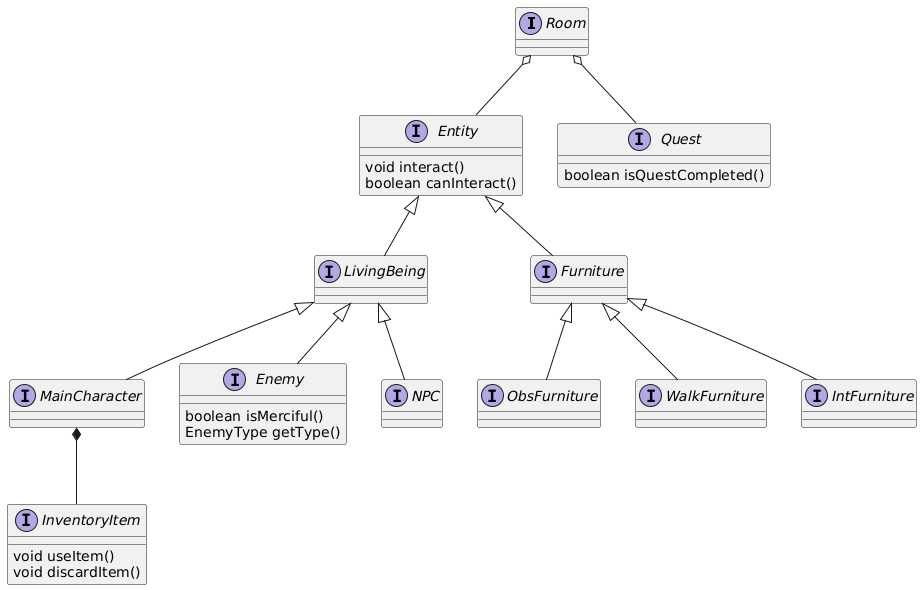
\includegraphics[width=\textwidth]{img/model.png}
	\caption{Schema UML del dominio applicativo}
	\label{img:model}
\end{figure}


\chapter{Design}

\section{Architettura}

Il software si basa sull’architettura MVC nella sua declinazione standard. In particolare, ogni elemento dell’architettura offre un unico entry point verso l’esterno, in modo che gli accessi alle sue funzionalità possano essere uniformi e consistenti, offrendo un ulteriore grado di incapsulamento.
%
\newline Il Model offre come proprio entry point l’interfaccia Room, che fa da scenario base per lo svolgimento della fase di esplorazione del gioco. All’interno della stanza infatti, sono presenti tutte le entità, che vengono modificate ad ogni tick del motore fisico tramite un metodo offerto dalla stessa Room, deputata a controllare anche se le singole entità siano in grado di muoversi al suo interno. 
%
\newline Il Controller, che conserva il riferimento alla stanza in cui attualmente si trova il gioco, gestisce al suo interno le transizioni di stato per le varie fasi del gameplay, interrogando la View per mostrare le interfacce corrette e richiedendo al Model eventuali modifiche. Il Controller è anche responsabile della temporizzazione dell’aggiornamento del motore di gioco, e della traduzione delle entità del Model in elementi rappresentabili correttamente dalla View.
%
\newline La View offre un entry point centrale da cui è possibile richiedere di mostrare le varie interfacce, o l’accesso ai loro riferimenti per chiamare procedure proprie di tali istanze. Nell’architettura realizzata, la View agisce come elemento passivo ricevendo i dati da mostrare dal Controller tramite opportune interrogazioni. La gestione dell’input permette alla View di comunicare particolari eventi al Controller, che li gestirà e ne rifletterà eventualmente gli effetti sul Model.
%
\newline Nella realizzazione dell’architettura MVC, modificare la View non impatta minimamente il Model, dal momento che è solamente il Controller a dialogare con questa componente. Dall’altro lato, il Controller potrebbe essere impattato da una modifica della View radicale (come per esempio trasformare la GUI attiva in un’interfaccia reattiva, oppure la rimozione dei suoni), mentre non sarebbe impattato da modifiche nelle tecniche implementative della GUI - come per esempio una modifica della libreria grafica - a patto che sia in grado di rispettare il contratto stabilito dalle due interfacce (ad esempio accettare gli stessi tipi di chiamate parametrizzate).


\begin{figure}[H]
	\centering{}
	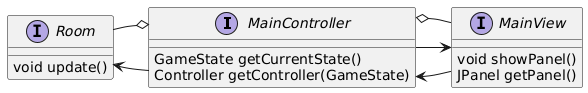
\includegraphics[width=\textwidth]{img/mvc.png}
	\caption{Schema UML degli entry point dei rapporti fra componenti di MVC}
	\label{img:mvc}
\end{figure}

\section{Design dettagliato}

\subsection{Mazuru Mihai}

\subsubsection{Furniture}
\paragraph{Problema}: Nella modellazione degli oggetti di arredo mi sono imbattuto nel problema 
di come realizzare diverse tipologie di arredi senza ripetizioni di codice. Questi oggetti 
sono caratterizzati da un nome, una descrizione, una posizione e un tipo, e invece si differenziano 
per le seguenti proprietà: attraversabilità e interattività.
\paragraph{Soluzione} Ho optato per l'implementazione del pattern \textit{Template Method}. 
L'ho applicato realizzando una classe astratta \textit{Furniture} che contiene la logica comune a 
tutti gli oggetti di arredo (con i corrispettivi getter) e i metodi astratti \textit{isWalkable()} e 
\textit{isInteractive()}. L'implementazione di questi metodi viene lasciata ad ogni sottoclasse.
Difatti la classe \textit{WalkableFurniture} definisce oggetti di arredo con i quali si può interagire e
che non ostacolano il passaggio delle entità viventi, mentre la classe \textit{ObstructingFurniture} 
definisce oggetti con caratteristiche diametralmente opposte (bloccanti e non interattivi) e 
invece la classe \textit{InteractiveFurniture} definisce oggetti con caratteristiche intermedie (bloccanti ed interattivi).
\newline La soluzione scelta consente inoltre l'estendibilità, facilitando la creazione di una nuova
ipotetica classe con oggetti attraversabili e non interattivi.

\begin{figure}[H]
	\centering{}
	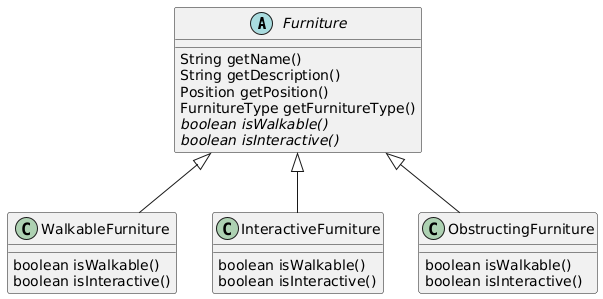
\includegraphics[width=\textwidth]{img/template.png}
	\caption{Schema UML dell'applicazione del pattern Template Method alla gerarchia delle Furniture.}
	\label{img:template}
\end{figure}

\paragraph{Problema} La creazione dei diversi oggetti di arredo attraverso una semplice "new" comporterebbe
l'aggiunta di dipendenze al nostro codice, rendendolo più difficile e tedioso da testare, 
complicando la sua estendibilità ed eventualmente la sua manuntenzione. 
\paragraph{Soluzione} Proprio per questo ho scelto di utilizzare il pattern \textit{Simple Factory} per la 
creazione degli arredi. Ho realizzato un'interfaccia che contiene i metodi per la creazione dei diversi
tipi di arredi. Questi metodi vengono implementati dalla sua sottoclasse, la quale è in grado di creare 
oggetti randomici, specifici oppure solo di un determinato tipo. Gli unici parametri richiesti sono il tipo
e la posizione dell'arredo, mentre le altre caratterische come il nome e la descrizione vengono gestite
internamente alla factory attraverso una mappa che contiene per ogni tipo diverso di arredo una descrizione unica.

\begin{figure}[H]
	\centering{}
	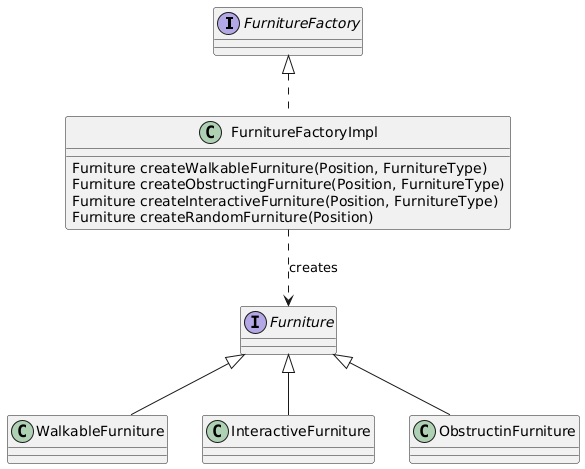
\includegraphics[width=\textwidth]{img/furnitureSimpleFactory.png}
	\caption{Schema UML dell'applicazione del patter Simple Factory per la creazione di Furniture.}
	\label{img:furnitureSimpleFactory}
\end{figure}

\subsubsection{Gestione panelli di gioco}

\paragraph{Problema} Il nostro progetto si articola in diversi momenti di gioco e il problema iniziale
era proprio quello di capire come gestire nel migliore dei modi il passaggio da una pannello di gioco ad 
un altro.
\paragraph{Soluzione} Per risolvere questo problema il gruppo ha scelto di creare una \textit{MainView} che
si sarebbe occupata della creazione del frame, della creazione dei vari pannelli di gioco e
delle transizione da un pannello all'altro.
Io mi sono occupato dell'implementazione e ho optato per l'utilizzo di \textit{CardLayout}, un manager layout
che permette di associare ad ogni pannello una stringa di testo, attraverso la quale sarà possibile far emergere
dalla "pila di carte" il pannello desiderato. L'invocazione del metodo per far emergere un certo pannello viene effettuata
dal corrispondente controller.
\begin{figure}[H]
	\centering{}
	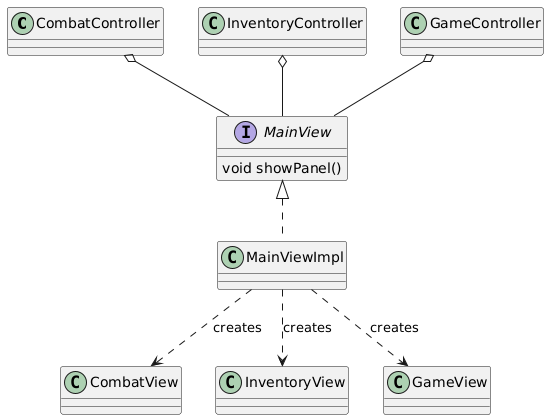
\includegraphics[width=\textwidth]{img/mainView.png}
	\caption{Schema UML che rappresenta MainView, alcuni pannelli di gioco, alcuni controller del gioco e le loro interazioni.}
	\label{img:mainView}
\end{figure}

\subsubsection{Gestione combattimento}

\paragraph{Problema} Il combattimento è uno dei momenti più importanti del gioco e la sua gestione 
in modo ottimale è fondamentale per garantire una gradevole esprienza all'utente. La gestione dei turni e la 
gestione delle azioni di combattimenti sono aspetti importanti per il raggiungimento di questo obiettivo.
\paragraph{Soluzione} Le possibili scelte all'interno della fase di combattimento sono: attaccare, chiedere pietà oppure
aprire l'inventario. Queste possibili azioni vengono gestite tramite un Action Listener che notifica
il \textit{CombatController}. Il controller in questione attraverso uno switch, al quale si accede solo se l'azione avviata
precedentemente è finita, delega la gestione dell'azione agli appositi metodi privati oppure delega il lavoro al controller
dell'inventario (nel caso si scelga di aprire l'inventario). 
I turni invece vengono gestiti in maniera automatica. Una volta che il giocatore ha attaccato, il nemico, se è ancora in vita, 
attacca subito a sua volta. L'unico caso in cui è il nemico ad attaccare per primo è quando al giocare viene negata
la richiesta di pietà e di conseguenza salta il turno.
Sono stati aggiunti dei \textit{Timer} per non accavallare le varie azioni e degli aggiornamenti testuli a fine di ogni azione, in modo da
rendere il combattimento più intrattenete. Questi aggiornamenti testuali, insieme alle caratteristiche dei combattenti, vengono
rese visibili e aggiornate attraverso una chiamata di "update" alla \textit{CombatView}. 
\begin{figure}[H]
	\centering{}
	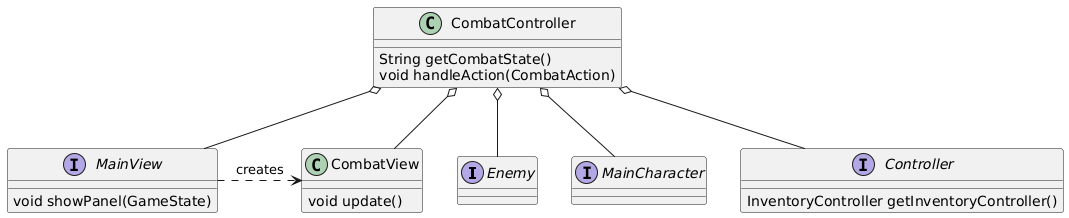
\includegraphics[width=\textwidth]{img/combatController.png}
	\caption{Schema UML che rappresenta il CombatController e le sue principali relazioni.}
	\label{img:combatController}
\end{figure}

\subsection{Kimi Osti}
Questa sezione è stata redatta facendo riferimento, oltre ai pattern presentati dalla Gang of Four, anche al libro \cite{nystrom2014}, presentato dal Prof. Alessandro Ricci durante il seminario Game as a Lab.

\subsubsection{Input da tastiera nella fase di esplorazione}
\begin{figure}[H]
	\centering
	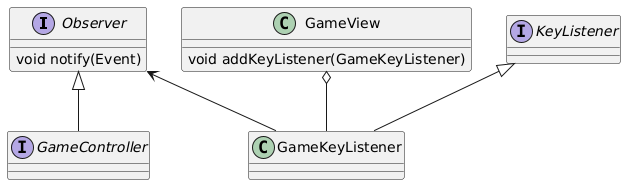
\includegraphics[width=\textwidth]{img/observer-gameview.png}
	\caption{Schema UML delle classi e interfacce coinvolte}
	\label{img:observer-gameview}
\end{figure}
\paragraph{Problema} Il giocatore comanda il personaggio principale tramite tastiera, e gli input devono essere catturati dal \textit{GameController}.
\paragraph{Soluzione} La collaborazione fra classi viene realizzata grazie al pattern \textit{Observer}. In particolare, la classe \textit{GameView} fa da observable, e tramite il \textit{KeyListener} registrato trasmette i propri eventi al \textit{GameController}, che fa da observer. In particolare, in questa soluzione viene sfruttato un \textit{GameKeyListener} che implementa l'interfaccia \textit{KeyListener}, filtrando i tasti di interesse per il gioco e traducendoli in un particolare \textit{Event}, enumerazione definita all'interno del progetto per tracciare gli eventi rilevanti all'applicazione. Grazie a questa enumerazione, gli eventi sono trattati ad alto livello e si permette facilmente estendibilità verso la funzionalità opzionale della riassegnabilità dei tasti, a patto di permettere al GameKeyListener di modificare la mappatura da evento di pressione del tasto ed \textit{Event}.

\subsubsection{Creazione e gestione dei componenti per l'interfaccia di esplorazione}
\begin{figure}[H]
	\centering
	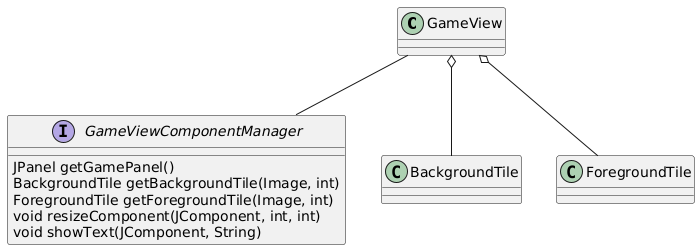
\includegraphics[width=\textwidth]{img/factory-gameview.png}
	\caption{Schema UML delle classi e interfacce coinvolte}
	\label{img:factory-gameview}
\end{figure}
\paragraph{Problema} Nell'interfaccia della fase di esplorazione, si deve renderizzare il contenuto della mappa, oltre a un banner contenente i comandi nella parte superiore dello schermo e un banner con eventuali messaggi di interazione nella fase inferiore. Ciò significa avere diversi pannelli, tutti accomunati dallo sfondo nero, e di cui i due superiori devono contenere eventualmente testo, mentre quelli centrali delle scene rappresentate dalla sovrapposizione di \textit{BackgroundTile} e \textit{ForegroundTile}
\paragraph{Soluzione} Per alleggerire l'implementazione di \textit{GameView} e renderla più comprensibile, si è creata una helper class in grado di gestire i componenti dell'interfaccia. In particolare, si sottolineano i metodi che fungono da Factory, ovvero i tre metodi \textit{getGamePanel}, \textit{getBackgroundTile} e \textit{getForegroundTile} che vengono usati per creare i componenti che andranno poi a formare l'interfaccia grafica nel suo complesso. Vengono inoltre definiti due metodi per ridimensionare i componenti e per mostrare il testo contenuto al loro interno.

\subsubsection{Gestione del Main Loop}
\begin{figure}[H]
	\centering
	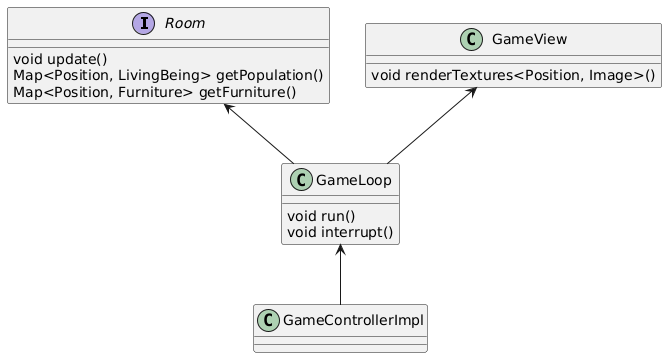
\includegraphics[width=\textwidth]{img/game-loop.png}
	\caption{Schema UML delle classi e interfacce coinvolte}
	\label{img:game-loop}
\end{figure}
\paragraph{Problema} Il Model, essendo presenti entità viventi all'interno della stanza, deve essere periodicamente aggiornato per rendere effettivo il movimento di tali entità, e in particolare il risultato dell'aggiornamento deve essere reso visibile all'utente tramite View.
\paragraph{Soluzione} All'interno di \textit{MainControllerImpl} viene istanziato il \textit{GameLoop}, un thread separato che si occupa di gestire la temporizzazione degli aggiornamenti del Model, come presentato nel Game Loop Pattern in \cite{nystrom2014}. In questo modo, la gestione dell'input rimane delegata a \textit{GameControllerImpl}, mentre la temporizzazione dell'aggiornamento viene gestita da \textit{GameLoop} per evitare dipendenze. Inoltre, la temporizzazione viene legata al tempo reale piuttosto che al tempo di CPU, per evitare rese diverse su processori di diverse potenze. \textit{GameLoop} è anche deputata di comandare a \textit{GameView} gli aggiornamenti necessari a rappresentare le modifiche del Model, e per motivi legati alla rappresentazione unitaria della posizione all'interno del Model l'aggiornamento della View viene effettuato di pari passo rispetto a quello del Model, anche se si sarebbe potuto svincolare per massimizzare il framerate indipendentemente dalla velocità di aggiornamento del Model. 
\newline Nello scenario del Game Loop pattern viene applicato anche il pattern dell'Update Method, sempre presentato in \cite{nystrom2014} e strettamente legato. In particolare, i metodi interessati sono \textit{update} in \textit{Room} e \textit{renderTextures} in \textit{GameView}.

\subsubsection{Individuazione delle texture}
\begin{figure}[H]
	\centering
	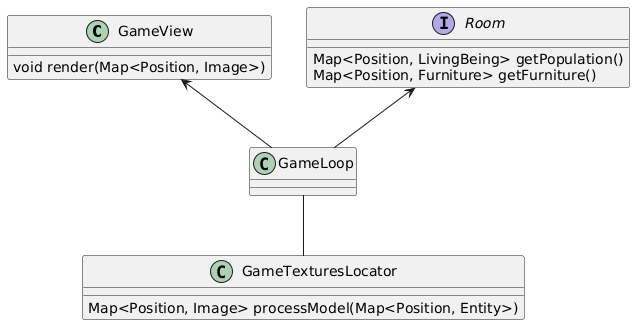
\includegraphics[width=\textwidth]{img/locator-game.png}
	\caption{Schema UML delle classi e interfacce coinvolte}
	\label{img:locator-game}
\end{figure}
\paragraph{Problema} Durante la fase di esplorazione del gioco, ad ogni frame, il contenuto della stanza deve essere renderizzato traducendo le entità del Model in elementi rappresentabili dalla View.
\paragraph{Soluzione} Per risolvere il problema riducendo al minimo le dipendenze, si è introdotta una classe che fa da Locator per le texture. In questo modo, il Controller, reificato in \textit{GameLoop}, può accedere al Model per interrogarlo sul contenuto della stanza, e inviare il contenuto del Model processato dal Locator alla View per il rendering. Ciò significa che il Main Loop rimane completamente agnostico rispetto al formato richiesto dalla View, delegando il compito di traduzione da classi di Model a risorse di View al Locator. In questo modo, una sostituzione anche in blocco della View comporterebbe necessità di modifica solo all'interno del Locator, evitando così di impattare Controller e Model.

\chapter{Sviluppo}

\section{Testing automatizzato}

Per quanto riguarda il testing automatizzato, si è sfruttata la libreria JUnit e si sono realizzati test su quasi tutte le classi di Model e Controller. Ciò è stato fatto per garantire il corretto funzionamento dell’applicazione, e per avere la certezza che gli eventuali problemi riscontrati durante il gioco non fossero dovuti a mancanze di logica implementativa, quanto a problematiche di visualizzazione. 
%
\newline La View, invece, è stata testata manualmente in fase di sviluppo, e poi in fase di collaudo del software, perché personalmente non siamo riusciti ad approfondire le dinamiche di testing automatizzato che avrebbero permesso di testare automaticamente anche quella parte del software.
%
\newline In linea generale, gli aspetti su cui il testing si è maggiormente soffermato sono stati i seguenti:

\begin{itemize}
	\item Generazione della mappa, movimento e interazioni al suo interno. Particolarmente, si è verificato che il movimento e le interazioni non generassero comportamenti imprevisti e che si riflettessero correttamente sugli aggiornamenti del Model.
	\item Combattimento. In particolare, il testing si concentra sul mantenimento dell’ordine dei turni per evitare comportamenti imprevisti, e sul corretto inserimento in inventario del bottino dei nemici sconfitti.
	\item Protagonista. In particolare, si è testato il sistema di gestione della vita del protagonista, così come del suo inventario. Nei controlli sull’inventario, si è verificato il corretto utilizzo degli oggetti curativi, così come delle armi e armature, per garantire comportamenti consistenti in fase di combattimento.
	\item Input utente. Si sono testati i Controller che svolgono la funzione di Observer, per garantire la corretta gestione degli input.
	\item Creazione delle istanze. Avendo fatto largo uso del Pattern Factory, si è deciso di testare i metodi di generazione degli oggetti per verificare l’effettiva consistenza delle istanze create e garantire prevedibilità in fase di gioco.
\end{itemize}

\section{Note di sviluppo}

\subsection{Kimi Osti}

Di seguito si presentano singoli esempi di uso di costrutti avanzati di Java. Ciò non impedisce che all'interno del codice appaiano più situazioni in cui vengono usati.
\begin{itemize}
	\item \textbf{Java Wildcards} al permalink \url{https://github.com/KimboCoffee/OOP23-relario/blob/d67fe167022e08cef63d110da0710154eb543292/src/main/java/it/unibo/oop/relario/utils/impl/GameTexturesLocator.java#L42}
	\item \textbf{Lambda Expressions e Optional} al permalink \url{https://github.com/KimboCoffee/OOP23-relario/blob/d67fe167022e08cef63d110da0710154eb543292/src/main/java/it/unibo/oop/relario/model/inventory/InventoryImpl.java#L40}
	\item \textbf{InputStream} al permalink \url{https://github.com/KimboCoffee/OOP23-relario/blob/d67fe167022e08cef63d110da0710154eb543292/src/main/java/it/unibo/oop/relario/view/impl/UserGuide.java#L54}
	\item \textbf{Gestione dei Thread} al permalink \url{https://github.com/KimboCoffee/OOP23-relario/blob/cb9e0fd37a803cebfb509ff1b08d7df99b5ee8fc/src/main/java/it/unibo/oop/relario/controller/impl/GameLoop.java}
\end{itemize}

\subsubsection{Codice reperito online}
Per la realizzazione della classe BackgroundTile (Permalink:  \url{https://github.com/KimboCoffee/OOP23-relario/blob/d67fe167022e08cef63d110da0710154eb543292/src/main/java/it/unibo/oop/relario/view/impl/BackgroundTile.java}) si è preso spunto da \href{https://coderanch.com/t/336043/java/Images-top}{questa pagina di forum online}.

\subsection{Mazuru Mihai}
\begin{itemize}
	\item \textbf{Stream}: Utilizzato per il recuperare il valore corrispondente ad una nota chiave in una mappa.
	Permalink \url{https://github.com/KimboCoffee/OOP23-relario/blob/d67fe167022e08cef63d110da0710154eb543292/src/main/java/it/unibo/oop/relario/view/impl/MainViewImpl.java#L84-L95}
    
	\item \textbf{Stream}: Utilizzato per filtrare gli arredamenti in base al loro tipo (Walkable, Obstructing, Interactive).
	Permalink \url{https://github.com/KimboCoffee/OOP23-relario/blob/d67fe167022e08cef63d110da0710154eb543292/src/main/java/it/unibo/oop/relario/model/entities/furniture/impl/FurnitureFactoryImpl.java#L128-L131}

	\item \textbf{Lambda function}: Utilizzato per l’Action Listener di JButton.
	Permalink \url{https://github.com/KimboCoffee/OOP23-relario/blob/d67fe167022e08cef63d110da0710154eb543292/src/main/java/it/unibo/oop/relario/view/impl/MenuView.java#L87-L109}

	\item \textbf{Optional}: Utilizzo per gestire i nemici all'interno degli arredamenti.
	Permalink \url{https://github.com/KimboCoffee/OOP23-relario/blob/d67fe167022e08cef63d110da0710154eb543292/src/main/java/it/unibo/oop/relario/model/entities/furniture/impl/WalkableFurnitureImpl.java#L12-L73}
\end{itemize}

\subsubsection{Codice preso da altri}
\textbf{Modellazione molteplici menu}: Utilizzo model per gestire molteplici menu.
Permalink \url{https://github.com/luca-casadei/OOP23-the-exiled/blob/3980cb23272808019d315d20593faae31b543f89/src/main/java/unibo/exiled/model/menu/MenuModelImpl.java#L6-L33}

\chapter{Commenti finali}

\section{Autovalutazione e lavori futuri}

\subsection{Mazuru Mihai}
Spero che il mio contributo all'interno del team sia stato significativo. All'inizio, a causa dell'ansia per questo progetto, ho avuto difficoltà a essere d'aiuto nelle fasi decisionali. Tuttavia, con il tempo, man mano che acquisivo maggiore confidenza con il progetto e con le persone con cui lavoravo, sono riuscito a sbloccarmi e a mettermi in gioco.

Mi auguro inoltre di aver trasmesso agli altri membri del gruppo la mia determinazione, dimostrando il mio impegno nel partecipare a ogni incontro e contribuendo attivamente alla realizzazione del MainController e della MainView.

Per quanto riguarda il resto del team, li considero colleghi straordinari e persone sempre disponibili, sia nel fornire chiarimenti che nel darmi una mano quando ne avevo bisogno.

\subsection{Kimi Osti}
Personalmente, questo è stato il primo progetto di gruppo di queste dimensioni a cui mi sono dedicato, e in particolare è stato il primo progetto a cui mi sono dedicato in ambito di videogiochi, tema che mi ha sempre molto affascinato e a cui vorrei dedicare anche la mia carriera futura. In particolare per questo motivo, ho trovato stimolante la fase di sviluppo del software e particolarmente gratificante riuscire a produrre un risultato finale funzionante.
\newline Per quanto riguarda lo sviluppo del software - guardando indietro alle fasi iniziali del progetto - posso dire di ritenermi abbastanza soddisfatto. Durante il corso del progetto ho principalmente appreso alcune delle dinamiche nello sviluppo di software di dimensioni più grandi rispetto ai soliti progetti individuali a cui mi ero dedicato in precedenza, e ho anche capito alcuni concetti che - prima di iniziare a lavorare su questo progetto - non avrei saputo affrontare. Pertanto, posso dire che questo progetto mi è servito individualmente a maturare ulteriormente, e che se dovessi tornare indietro probabilmente lavorerei in modo diverso non tanto per modificare il risultato finale (che si è dimostrato abbastanza vicino a quello che mi ero prefigurato prima di iniziare il lavoro), quanto più in virtù delle dinamiche che ho appreso durante il lavoro e che avrebbero permesso di produrre software in maniera più efficiente.
\newline Per quanto riguarda le dinamiche di gruppo, posso dirmi abbastanza soddisfatto, soprattutto per il fatto che, anche se in alcune fasi vi sono state divergenze di vedute su alcune tematiche, non si sia mai arrivati a situazioni critiche che abbiano pregiudicato lo svolgimento del lavoro. Fin da prima di presentare il progetto, però, sono stato io a presentare l'idea su cui poi si è sviluppato il gioco, e durante il progetto - complice la fiducia che i miei compagni hanno riposto in me - ho assunto il ruolo di "coordinatore" del lavoro. Questo ha però inevitabilmente significato che gran parte delle idee su cui si basa il modello del gioco siano arrivate da me, e che poi io mi sia trovato - soprattutto nelle fasi finali - ad affrontare personalmente le fasi di sviluppo più delicate, come per esempio la soluzione di possibili bug sottolineati dagli strumenti di analisi statica del codice oppure la soluzione del problema di mancato caricamento delle risorse che si è presentata quando abbiamo assemblato il jar per la consegna finale.
\newline Nel complesso però, mi sento di dire che il risultato finale rispecchia abbastanza l'idea che avevo del gioco prima di iniziare lo sviluppo, e che ho trovato stimolante il processo di realizzazione. Per come è strutturato il software ci sarebbe margine per allargarlo e portarlo a qualcosa di più di una demo da qualche minuto, anche se dubito che possa accadere. D'altro canto, personalmente vedo rafforzata la mia passione verso il mondo dello sviluppo di videogiochi, e sono volenteroso di portare avanti questa passione anche con progetti personali che possano permettermi di approfondire ulteriormente parti dello sviluppo che per motivi di suddivisione del lavoro ho toccato meno.

\section{Difficoltà incontrate e commenti per i docenti}

\appendix
\chapter{Guida utente}

Durante il gioco l'utente deve attraversare delle stanze, in cui deve completare eventuali quest.
\newline Nei menu, come nel combattimento, l'input viene accettato tramite mouse, con dei clic sui bottoni che rappresentano l'azione desiderata.
\newline Durante l'esplorazione, il giocatore si sposta con WASD, interagisce con la cella che guarda con E e apre l'inventario con I.
\newline Per superare ciascuna stanza, deve completare la quest(se presente) che gli viene presentata dall'NPC fermo all'entrata. Dopo aver completato la quest, deve raggiungere il tappeto situato a destra della stanza, e interagire da sopra la casella al suo entremo destro per proseguire nella stanza successiva.
\newline All'interno dell'inventario, gli oggetti vengono scelti con le frecce verticali, e si possono equipaggiare con ENTER oppure scartare con BACKSPACE. Un oggetto che non abbia effetto, quando usato, viene "consumato" e non risulta quindi piu' disponibile.

\bibliographystyle{alpha}
\bibliography{report}

\end{document}
